%==========================================================================
\section{The Quartet Instruments} \label{introduction}

\begin{center}
\begin{tabular}{cc}
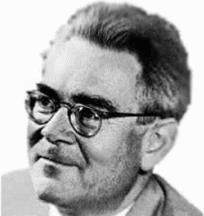
\includegraphics[scale=.5]{reichenbach_med.jpg} &
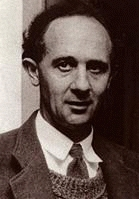
\includegraphics[scale=.6]{prior.jpg} \\
\emph{Hans Reichenbach}
& \emph{Arthur Prior}\\
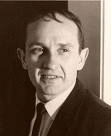
\includegraphics[scale=.8]{montague.jpg} &
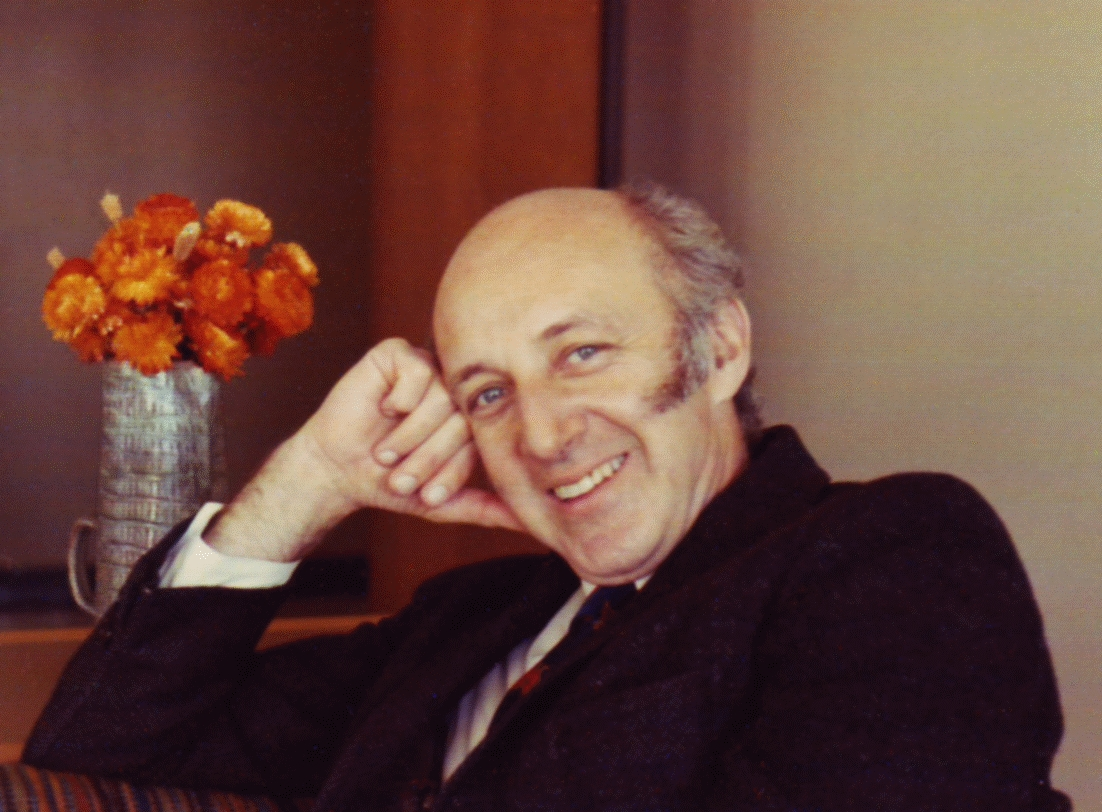
\includegraphics[scale=.1]{henkin73.jpg}\\
\emph{Richard Montague}
&\emph{Leon Henkin}
\end{tabular}%
\end{center}%

Hybrid type theory and its completeness proof will be presented in the next
sections.

Before this, in this introduction, a brief historical revision of the
important concepts that this article is about and of their four mentioned
inventors is presented.

\subsection{Reichenbach: Tense Referential Analysis}

Hans Reichenbach in his book \emph{Elements of Symbolic 
Logic}~\cite{Reichenbach1947} included two chapters about the linguistic applications
of logic. It is especially relevant its treatment of tenses in natural
language. \emph{``Tenses determine time with reference to
the time point of the act of 
speech''}~\cite{Reichenbach1947} for him. He represented tenses in terms of reference with respect to
three temporal points: \emph{the point of speech} (S), \emph{the point
of event} (E), and \emph{the point of reference} (R). The point of speech
is the time at which the sentence is uttered; the point of event is the time
at which the event spoken of takes place. If we were to use only points S
and E, there are three possibilities for that point of event:
\emph{``before the point of speech''},
\emph{``simultaneous with the point of speech''}, 
and \emph{``after the point of speech''}. Hence, with these two kind of points only three
general tenses could be explained (past, present and future) and, as
Reichenbach pointed out, ``the number of verb tenses is
obviously greater''; in particular, there are tenses
concerning time order for two events. This is why he introduced \emph{the
point of reference}, a contextually determined time also present in tenses,
let us illustrate it with two examples.

When we say \emph{``Alba had sung''} there
is a clear intuition about some past time between 
\emph{the point of speech} and \emph{the point of event} when the singing event occurred. For
instance, we are telling our friends that we traveled to Barcelona to
attend Alba's concert but arrived too late, after Alba did sang. This
contextually determined past time is the point of reference. Accordingly,
the three dimensional representation of time ordering of the sentence 
\emph{``Alba had sung''} is E--R--S (where the
point of event is past the point of reference, which in turn is past the
point of speech). When we uttered \emph{``Alba
sang''}, we express that a singing event takes place at
some contextually determined past time, and its Reichenbach's tense
representation is E,R--S; that is, \emph{the point of event} and 
\emph{the point of reference} coincide and it is past the point of speech. In both
examples, the point of reference is some past time determined by the
context. In Figure~\ref{fig1} Reichenbach's representation of the English tenses by
using the three time markers is showed.

\begin{figure}[h]
\begin{center}
\begin{tabular}{|l|l|l|}
\hline
Structure & Name & \emph{Example} \\ \hline
E-R-S & Pluperfect & \emph{Alba had sung} \\ \hline
E,R-S & Past & \emph{Alba sang} \\ \hline
R-E-S or\ R-S,E or R-S-E & Future in the past & \emph{Alba would sing} \\ 
\hline
E-S,R & Perfect & \emph{Alba has sung} \\ \hline
S,R,E & Present & \emph{Alba sings} \\ \hline
S,R-E & Prospective & \emph{Alba is going to sing} \\ \hline
S-E-R or S,E-R or\ E-S-R & Future perfect & \emph{Alba will have sung} \\ 
\hline
S-R,E & Future & \emph{Alba will sing} \\ \hline
S-R-E & Future in the future & \textquestiondown ? \\ \hline
\end{tabular}%
\end{center}
\caption{Figure 1: Reichenbach's analyses of the tense forms of English.}\label{fig1}
\end{figure}

Reichenbach's analysis has had many objections; for instance, his use of
three different diagrams to represent the future in the past and the future
perfect tenses, or his little subtle analysis of the present perfect (simply
expressing that the point of reference corresponds to point of speech).
However, the \emph{point of reference} is a historically relevant
innovation. Without some way of expressing this kind of temporal reference,
many temporal constructions cannot be represented.

\subsection{Prior: Tense Logic}

Arthur Prior invented the orthodox tense logic, as a simple kind of modal
logic for reasoning about time. Prior introduced the internal perspective of
modal logics, where formulas are evaluated at some particular point within
models, as a way of capturing the \emph{``time-situated''} information. As the central
elements of his tense logic, he defined the $F$ and $P$ modalities (meaning 
\emph{``at some future time''}, and 
\emph{``at some past time''}, respectively). Let
us see how it works. Consider the present-tense English sentence 
\emph{``Alba sings''} and suppose that the
propositional symbol $\mathit{alba.sing}$ is its representation in tense logic. Now
consider the expression obtained by prefixing this with the $P$ operator, $%
P\ \mathit{alba.sing}$, which is true at a time $t$ if Alba does indeed sing at some
time $t_{0}$ before that $t$. However, this representation means that at
some completely unspecified past time Alba did sing, while the uttered
sentence \emph{``Alba Sang''} means that at some particular, contextually
determined, past time Alba did sing. Comparing with Reichenbach's analysis
Prior's representation captures only part of the meaning of the past-tense,
failing to capture the reference to specific times.

The \emph{time of speech} concept is fundamental to the internal
perspective and it fits perfectly with Prior's tense logic. It is simply the
particular time at which we evaluate a formula in a given model. It is also
fundamental the \emph{time of event} concept. In Prior's representation,
prefixing $\varphi $ to form $P\varphi $ or $F\varphi $ locates the point of
event to the past of \emph{the point of speech} or to the future of 
\emph{the point of speech}, respectively. Thus, Reichenbach's point of
speech and point of event are compatible with Prior's views of internal
perspective of tense logic. However, this is not the case for \emph{the
point of reference}. In the chapter 
\emph{``Precursors of tense-logic''} in his \emph{Past, Present and
Future}~\cite{Prior1967}, Prior dedicates a section to
Reichenbach's time of reference. Prior simply rejected Reichenbach's scheme
objecting among others that it did not cover new more complicated tenses as 
\emph{``I shall have been going to see John''}, \fixme{unclear and not structured} where there are two points of references
(S-R2-E-R1) and then the point of speech could be seen as the 
\emph{first} point of reference. He also
explained his own solution: the systematic definition of complex tenses in
terms of simpler ones. The central concept of 
\emph{``presentness''} as the simplest tense is fundamental in this
systematic construction. Tensed utterances can be formed by using some
modifier to the \emph{``timeless propositional
context''}. Prior is thinking about some kind of idea of
\emph{``presentness''} as 
\emph{``timeless context''} and modifiers
operators dealing with past and future.

\fixme{dangling}Prior's orthodox tense logic is very interesting and useful but it is not
able to capture the natural language tense nuances and the complexity of
real tense information.

\subsection{Montague: Intensional Logic}

Richard Montague thought that there is not an important theoretical
difference between natural languages and logical formal languages. Moreover.
In his \emph{``Universal 
Grammar''}~\cite{Montague1970}, he tried to develop a universal syntax and semantics that
acted as the framework for both types of languages. In his
\emph{``The Proper Treatment of Quantification in Ordinary
English''}~\cite{Montague1973}, Montague tried to present
syntax and semantics of a fragment of English rigorously. To do this, he
presented a logic system (where, in particular, rules of the tenses are
formalized) which he called \emph{Tense Intensional Logic}. He used Prior's 
$F$ and $P$ operators in that tensed variant of his Intensional Logic. There,
the central elements are types, used to capture the information on analysis
trees.

To interpret a linguistic expression is to assign intentions instead of
denotations, for him. An interpretation structure is of the kind 
$\langle \mathcal{A},I\rangle$ were $I$ is the \emph{set of
time moments} ($I$ is lineally ordered), where formulas can have different
denotations of truth values in different instants $i\in I$. Thus, for each 
$i\in I$, there would be a model $\langle \mathcal{A},i\rangle$.
\fixme{unclear}Whereas the interpretation $\langle \mathcal{A},I\rangle $ assign
intentions (functions from $I$ in the truth values or denotation sets) to
each expression or formula. Montague's idea is to conceive tenses as acting
on the intentions of the formulas instead of acting on the 
extensions~\cite{Montague1973}; \fixme{unclear} for instance, the truth value of a linguistic expression in
past tense, that is, its value in an instant $i$, depends on the values in
instants different from $i$.\fixme{Section too short.}

\subsection{Henkin: Completeness of Type Theory}

Right at the introduction of his paper ``Completeness in the
theory of types''~\cite{Henkin1950}, Henkin recalls the
known facts on the completeness/incompleteness issue, at that moment:

\begin{itemize}
\item The completeness of the first order calculus (G\"{o}del 1930): 
\emph{``\ldots each formula of the calculus is a formal theorem which
becomes a true sentence under one of a certain intended class of
interpretation of the formal system.''}

\fixme{\tiny In various parts this style of mixing quotes with text is used.  
The idea of using parts of the original paper (if indeed the quotes are direct
from the paper) is interesting, but I don't like 
the result?  Any idea?}
\item The incompleteness of the second order calculus (G\"{o}del 1931): 
\emph{``\ldots no matter what (recursive) set of axioms are
chosen, the system will contain a formula which is valid but not a formal
theorem.''} To interpret the language we use standard models where
\emph{``\ldots the individual variables are interpreted as ranging over an (arbitrary)
domain of elements while the functional variables of degree n range over all
sets of ordered n-tuples of individuals.''}
\end{itemize}

Leon Henkin studied incompleteness problems of higher order systems, like
the already mentioned G\"{o}del's incompleteness problem. G\"{o}del had
shown how to construct logically valid sentences (in standard models)\ which
were no formal theorems of the second order calculus. The problem persists in
any possible calculus: \emph{``no matter what (recursive)
set of axioms are chosen\ldots valid but not a formal theorem''}.

In~\cite{Henkin1950}, he explained the key point to have
completeness in higher order systems: \emph{``\ldots there is a
wider class of models \ldots redefine the notion of a valid formula\ldots second
order calculus is complete: a formula is valid if and only if it is a formal
theorem''}.

How did Henkin prove in his doctoral dissertation, in 1947, the completeness
theorem for type theory?

A very quick answer to this question is: by changing the semantics and hence
the logic. Let's see the second order case. We have $\mathcal{SS}$, the class of standard structures, and accordingly, we find $\VAL_{\mathcal{SS}}$, the set of validities in the class. We know that there is
no complete calculus for $\VAL_{\mathcal{SS}}$, since this set is
not recursively enumerable. But even knowing that there is no calculus in
the standard sense, we have certain axioms and rules which are sound and so
we define a calculus $\CAL$.

Since the set $\THEO$ of logical theorems is a proper subset of 
$\VAL_{\mathcal{SS}}$ , in order to get the right semantics for it, we
need to widen the class of structures to reduce the set of validities (the
wider the class, the smaller the set, because to be valid in a wider class
of structures a sentence needs to pass more, shall we say, 
\emph{``quality controls''}). We are very
restricted when asking the relational universes of any model to contain all
possible relations ---\emph{i.e.}, structures where $A_{n}=\mathcal{\wp }%
A^{n}$, for all $n$--- If we also allow non-standard structures ---\emph{i.e.}, structures where $A_{n}\subseteq \mathcal{\wp }A^{n}$, for all $n$ , but
for some $m$, $A_{m}\neq \mathcal{\wp }A^{m}$--- then the set of validities
in the very large class of structures which includes both classes is
considerably reduced. Apart from being a subset of the power set of the 
$n$-ary cartesian product of the universe of individuals, if we do not impose
any other condition on the universes of a structure, it may well happen that
it fails to contain certain relations that are definable in the structure
using second order formulas: This means the comprehension schema does not
necessarily hold. That is why we need structures where the relational
universes obey certain closure conditions: \emph{Henkin's general models}.

With the semantics of general structures, completeness (in both weak and
strong senses), L\"{o}wenheim-Skolem and all these theorems can be proved as
in first order logic. In fact, he first proved the completeness of type
theory and later on found a way to apply a similar method for first order
logic.

In his ``The discovery of my completeness
proofs''~\cite{Henkin1996} Henkin explained the real
process for him to invent his \emph{``general
models''} to interpret the pure functional calculus of
second order. His idea was that G\"{o}del`s valid (in standard models) but
not provable sentences were very special; and that by simple redefining what
a valid formula is, these troubled formulas could not be valid anymore. The
proof of Henkin's completeness theorem for higher order logic gives a
general method for constructing such general models, and, in particular,
what is now more important for us, a detailed proof of completeness with
respect to general models is done for a logical system of infinite order in
the form of a theory of types.
\fixme{\tiny not linked to the previous sections. Use more strongly the link 
with Montague.}
